\documentclass[hyperref={pdfpagelabels=false},usepdftitle=false]{beamer}
\usepackage{../templates/myStyle}

\begin{document}
\selectlanguage{ngerman}

\title{\titleText}
%\subtitle{Pixelweise Klassifikation von Straße}
\author{\tutor}
\date{22. Juli 2015}
%\subject{Programmieren}

\frame{\titlepage}

\frame{
    \frametitle{Contents}
    \setcounter{tocdepth}{1}
    \tableofcontents
    \setcounter{tocdepth}{2}
}

%\AtBeginSection[]{
%    \InsertToC[sections={\thesection}]  % shows only subsubsections of one subsection
%}

%!TEX root = Abschluss-ML-Prak-2015.tex
\section{Worum es geht}

\subsection{Die Aufgabe}

\begin{frame}{Die Aufgabe}
    \begin{itemize}
        \item \textbf{Eingabe}: Bilder, die von einer Kamera aus Fahrersicht
              aufgenommen wurden
        \item \textbf{Ausgabe}: Ein Bild gleicher Größe, wo jedes Pixel
              entweder schwarz ist (wenn der Klassifikator denkt es ist Straße)
              oder weiß ist (wenn dem) nicht so ist.
    \end{itemize}
\end{frame}

\begin{frame}{Die Daten}
    \href{http://www.cvlibs.net/datasets/kitti/eval_road.php}{KITTI Road Estimation dataset}
    \begin{itemize}
        \item Daten-Bilder der Größe $[1226, \dots, 1242] \times [370, \dots, 376]$,
              8-bit RGB
        \item Label-Bilder der selben Größe; 8-bit RGB mit 2 Farben
        \item 289 Trainingsbilder
        \item 290 Testbilder
    \end{itemize}
\end{frame}

\framedgraphic{Daten}{../images/umm_000000.png}
\framedgraphic{Labels}{../images/umm_road_000000.png}
\framedgraphic{Overlay}{../images/um_000000-overlay.png}
%!TEX root = Abschluss-ML-Prak-2015.tex
\section{Paper}

\subsection{Paper}

\begin{frame}{Paper}
    \begin{itemize}
        \item \href{http://arxiv.org/abs/1411.4038}{Fully Convolutional Networks for Semantic Segmentation}:
              Jonathan Long, Evan Shelhamer, Trevor Darrell
        \item pixelwise segmentation of multiple classes
    \end{itemize}
    
   
\end{frame}

\framedgraphic{Paper - Results}{../images/paper_results.png}
\framedgraphic{Paper - Heatmap}{../images/paper_heatmap.png}
\framedgraphic{Paper - Deconvolution}{../images/paper_dc.png}

%!TEX root = Abschluss-ML-Prak-2015.tex
\section{Unser Ansatz}
\subsection{Unser Ansatz}

\begin{frame}{Klassifikation - Sliding Window}
\begin{minipage}{0.59\textwidth}
\begin{itemize}
\item Klassifiziere mittigen Pixel der Eingabe \\
\item Laufe über das Bild (Sliding Window) \\
\item Überspringe Pixel zur Beschleunigung
\end{itemize}
\end{minipage}
\begin{minipage}{0.39\textwidth}
	\flushright
      
\includegraphics[]{../images/models/sliding_window.png}
\end{minipage}


\visible<2->{
	 \begin{center}
	 \only<1-2> {
        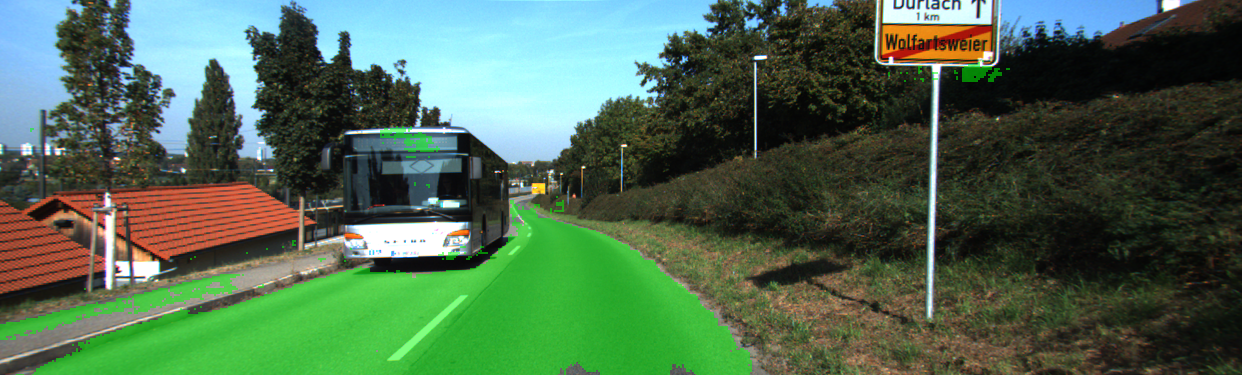
\includegraphics[scale=0.25]{../images/models/testing2-um_32_sliding_stride2.png}
      }
	 \only<3> {
        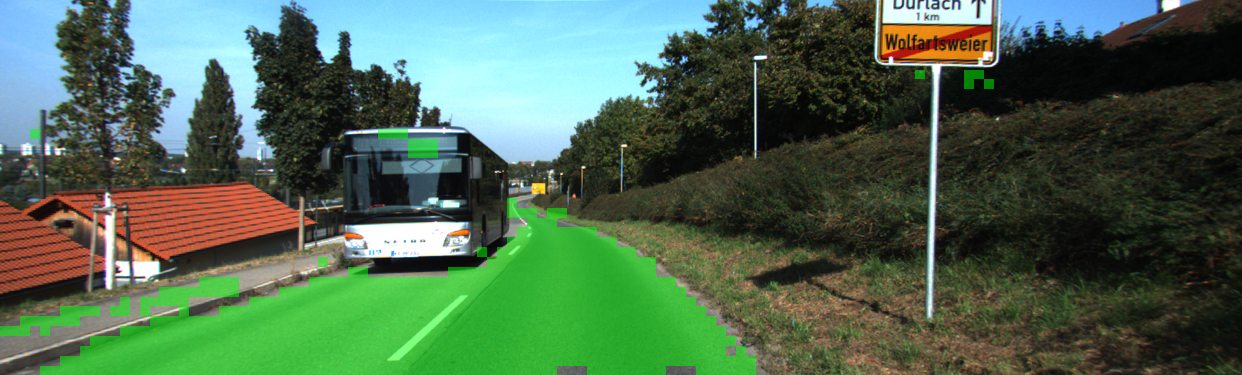
\includegraphics[scale=0.25]{../images/models/testing2-um_32_sliding_stride10.png}
      }
     \end{center}
     }
\end{frame}

\begin{frame}{Regression - Patch Evaluation}
\begin{minipage}{0.59\textwidth}
\begin{itemize}
\item Nutze Regression und Mean Squared Error Zielfunktion \\
\item Erhalte Information pro Pixel
\item Füge Bild zusammen \\
\end{itemize}
\end{minipage}
\begin{minipage}{0.39\textwidth}
	\flushright
      
\includegraphics[]{../images/models/fully-conv.png}
\end{minipage}


\visible<2->{
	 \begin{center}
	 \only<1-2> {
        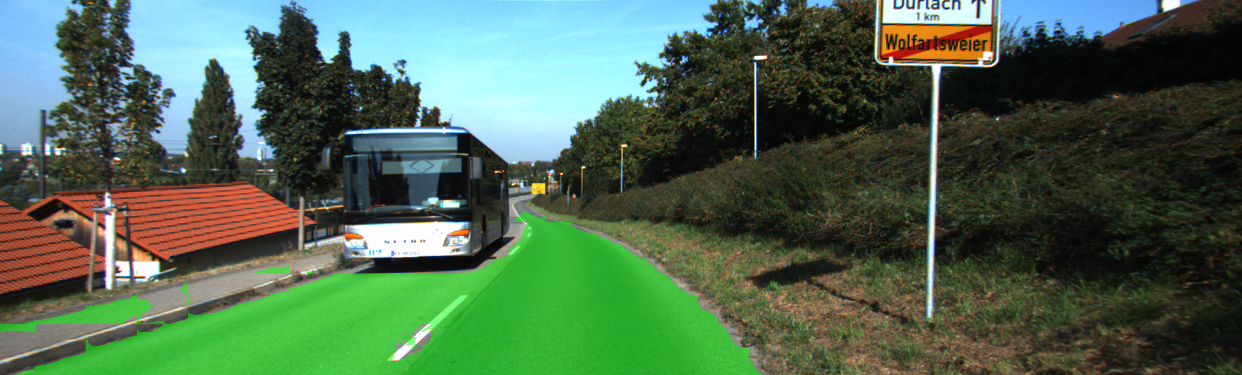
\includegraphics[scale=0.25]{../images/models/testing2-um_32_conv_stride51.png}
      }
	 \only<3> {
        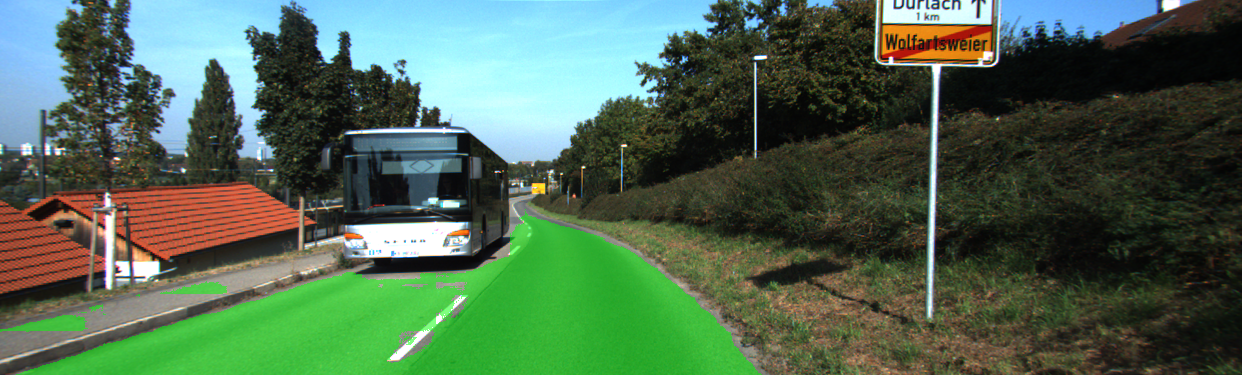
\includegraphics[scale=0.25]{../images/models/testing2-um_32_conv_stride37.png}
      }
     \end{center}
     }
\end{frame}

\begin{frame}{Aufbau unserer Neuronale Netze}
	\centering
\begin{minipage}{0.49\textwidth}
\centering
Klassifikationsnetz

\begin{itemize}
\item Input Layer $51 \times 51 \times 3$
\item 2 Conv Layer mit \\ 10 Filtern $5 \times 5$
\item 1 Pooling Layer
\item 1 Output Layer $1 \times 1$
\vspace{2.5em}
\end{itemize}
\end{minipage}
\begin{minipage}{0.49\textwidth}
\centering
Regressionsnetz

\begin{itemize}
\item Input Layer $51 \times 51 \times 3$
\item Conv Layer mit \\ 10 Filtern $3 \times 3$
\item Conv Layer mit \\ 1 Filtern  $51 \times 51$
\item Reshape Layer
\item 1 Output Layer $51^2 \times 1$
\end{itemize}

\end{minipage}

\end{frame}
%!TEX root = Abschluss-ML-Prak-2015.tex
%SEBASTIAN
\section{Ergebnisse}

\subsection{Ergebnisse}

\begin{frame}{Ergebnisse-Convolutional Layer}
    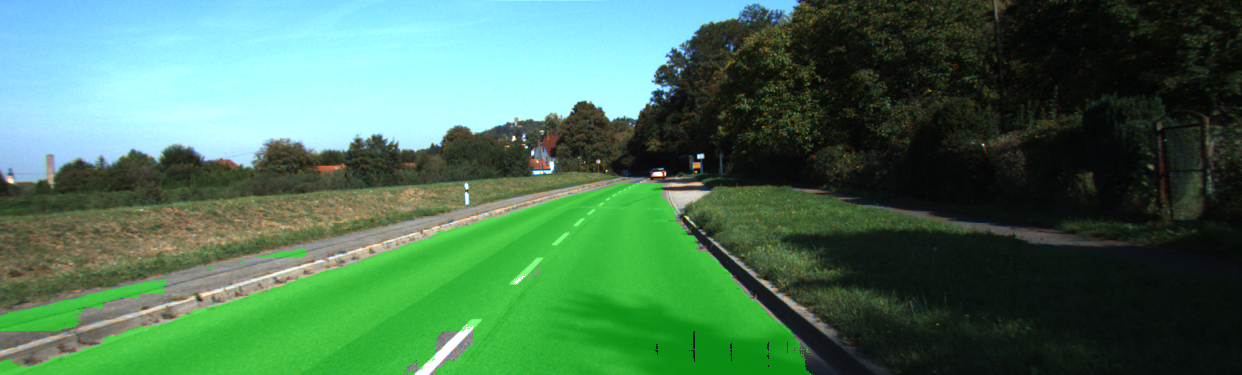
\includegraphics[scale=0.2]{../images/Convolutional/um_000014+-overlay-fully-49-patch.png}
\end{frame}

 \begin{frame}{Ergebnisse-Convolutional Layer}
    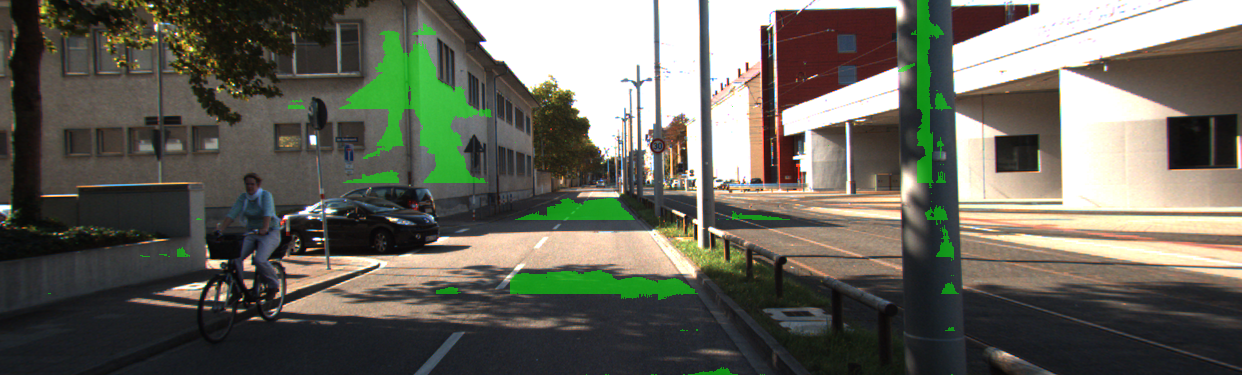
\includegraphics[scale=0.2]{../images/Convolutional/um_000066-overlay-fully-49-patch.png}
 \end{frame}

\begin{frame}{Vergleich}

      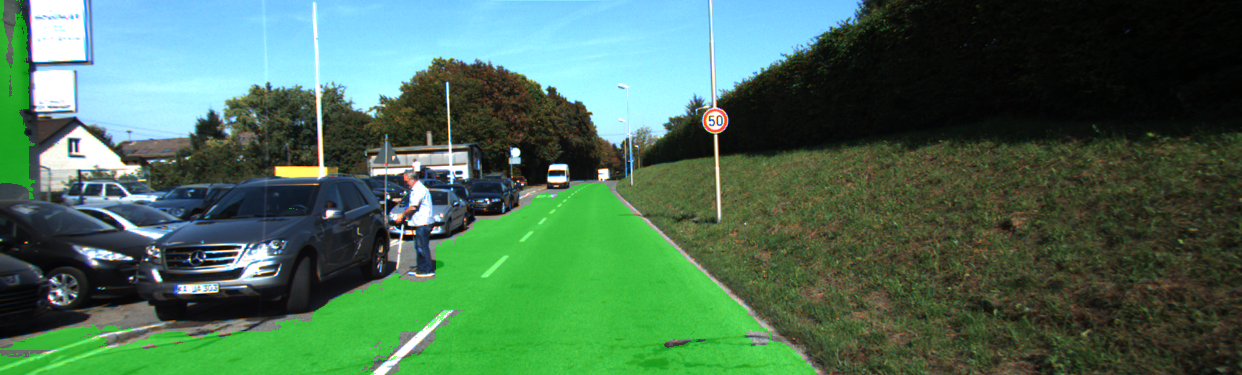
\includegraphics[scale=0.2]{../images/Convolutional/um_000014-overlay-fully-49-patch.png}
         \vspace{0.1cm}
    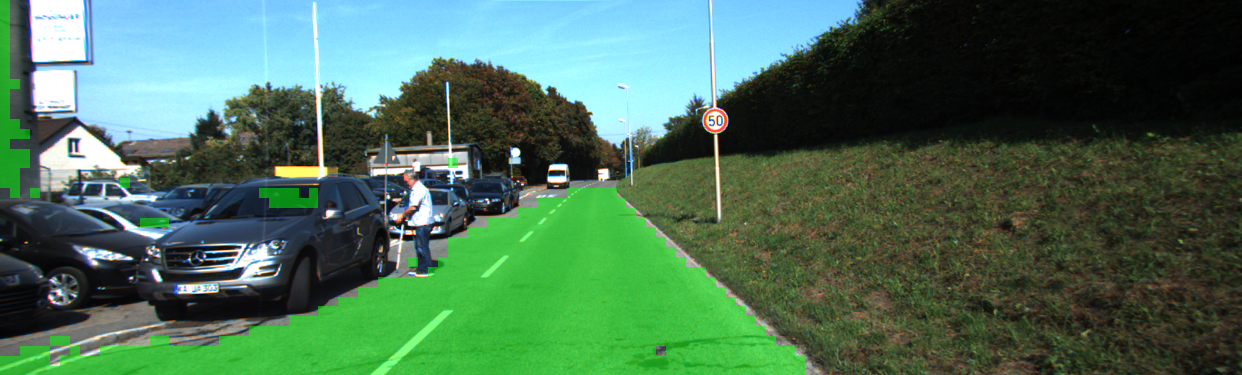
\includegraphics[scale=0.2]{../images/Convolutional/um_000014-overlay.png}

\end{frame}

\begin{frame}{Vergleich}

      False Positive Negative .....

\end{frame}

\begin{frame}{Laufzeiten}

      False Positive Negative .....

\end{frame}

\begin{frame}{Video}

      Video

\end{frame}

\section{Ausblick}
\subsection{Ausblick}
\begin{frame}{Ausblick}
    \begin{itemize}
        \item Wegen zu wenig RAM keine groesseren Patches
        \item Neuronales Netz verbessern
        \item Effizienteres Zusammensetzten der Patches
        \item Mehr Daten (Lens flare, Beleuchtung)
    \end{itemize}

\end{frame}
%!TEX root = Abschluss-ML-Prak-2015.tex
\section*{Ende}
\subsection{Ende}
\subsection{Quellen}
\begin{frame}{Bildquellen}
    \begin{itemize}
        \item \href{http://arxiv.org/abs/1411.4038}{Paper - Results and Heatmap} by Jonathan Long, Evan Shelhamer, Trevor Darrell
    \end{itemize}
        \begin{itemize}
        \item \href{https://swarbrickjones.wordpress.com/2015/04/29/convolutional-autoencoders-in-pythontheanolasagne/}{Paper - Deconvolution} by Mike Swarbrick Jones
    \end{itemize}
\end{frame}

\framedgraphic{Danke für die Aufmerksamkeit!}{../images/um_000000.png}

\end{document}
